\documentclass[12pt,a4paper]{article}


\usepackage{geometry}
\usepackage{fancyhdr}
\usepackage{enumitem}
\usepackage{lipsum} 
\usepackage{graphicx} 
\usepackage{tabularx}
\usepackage{colortbl}

\usepackage[hidelinks]{hyperref}

\usepackage{placeins}
\definecolor{lightgray}{gray}{0.9}

\usepackage{listings}
\usepackage{xcolor}
\usepackage{listings}
\usepackage{xcolor}
\usepackage{graphicx}
\usepackage{subcaption} 



\definecolor{mybg}{RGB}{248,248,248}
\definecolor{keygray}{RGB}{150,75,0}       
\definecolor{valueblue}{RGB}{0,102,204}   
\definecolor{stringpurple}{RGB}{128,0,128}
\definecolor{coloncolor}{RGB}{100,100,100}

% JSON 
\lstdefinelanguage{jsonstyled}{
    basicstyle=\ttfamily\small,
    backgroundcolor=\color{mybg},
    breaklines=true,
    showstringspaces=false,
    frame=single,
    literate=
     *{:}{{{\color{coloncolor}:}}}{1}
      {,}{{{\color{coloncolor},}}}{1}
      {"}{{{\color{keygray}"}}}{1}
      {[}{{{\color{black}[}}}{1}
      {]}{{{\color{black}]}}}{1}
      {0}{{{\color{valueblue}0}}}{1}
      {1}{{{\color{valueblue}1}}}{1}
      {2}{{{\color{valueblue}2}}}{1}
      {3}{{{\color{valueblue}3}}}{1}
      {4}{{{\color{valueblue}4}}}{1}
      {5}{{{\color{valueblue}5}}}{1}
      {6}{{{\color{valueblue}6}}}{1}
      {7}{{{\color{valueblue}7}}}{1}
      {8}{{{\color{valueblue}8}}}{1}
      {9}{{{\color{valueblue}9}}}{1},
}



\usepackage{xcolor}
\usepackage{listings}


\definecolor{codebg}{RGB}{248,248,248}       
\definecolor{codekeyword}{RGB}{0,0,180}     
\definecolor{codecomment}{RGB}{0,128,0}     
\definecolor{codestring}{RGB}{163,21,21}    
\definecolor{codeid}{RGB}{0,0,0}            

\lstdefinestyle{classicpython}{
    language=Python,
    backgroundcolor=\color{codebg},
    basicstyle=\ttfamily\small,
    commentstyle=\color{codecomment}\itshape,
    keywordstyle=\color{codekeyword}\bfseries,
    stringstyle=\color{codestring},
    identifierstyle=\color{codeid},
    showstringspaces=false,
    breaklines=true,
    frame=single,
    tabsize=4
}

\usepackage{listings}
\usepackage{xcolor}

\lstdefinestyle{classiclambda}{
    language=Python,
    basicstyle=\ttfamily\small,              
    keywordstyle=\color{blue!70}\bfseries,  
    commentstyle=\color{gray},               
    stringstyle=\color{green!60!black},      
    showstringspaces=false,                  
    numbers=none,                            
    frame=single,                            
    rulecolor=\color{gray!50},               
    backgroundcolor=\color{gray!5},          
    captionpos=b,                            
    tabsize=4,
    breaklines=true,
    escapeinside={(*@}{@*)},                 
    morekeywords={lambda, map, filter, reduce}, 
}

\usepackage{listings}
\usepackage{xcolor}


\definecolor{sqlbg}{RGB}{250,250,250}         
\definecolor{sqlkeyword}{RGB}{0,102,204}      
\definecolor{sqlidentifier}{RGB}{153,0,153}   
\definecolor{sqlstring}{RGB}{0,153,0}         
\definecolor{sqlframe}{RGB}{200,200,200}      

% SQL
\lstdefinelanguage{maevesql}{
    language=SQL,
    morekeywords={SELECT, FROM, WHERE, AND, OR, NOT, IN, LIKE, IS, NULL, ORDER, BY, GROUP, HAVING, AS, DISTINCT},
    sensitive=false,
    alsoletter={_},
    morecomment=[l]{--},
    morestring=[b]',
}

% SQL
\lstdefinestyle{maevesql}{
    language=maevesql,
    basicstyle=\ttfamily\small,
    keywordstyle=\color{sqlkeyword}\bfseries,
    identifierstyle=\color{sqlidentifier},
    stringstyle=\color{sqlstring},
    backgroundcolor=\color{sqlbg},
    frame=single,
    rulecolor=\color{sqlframe},
    showstringspaces=false,
    breaklines=true,
    captionpos=b,
}

\usepackage{listings}
\usepackage{xcolor}

\lstset{
  basicstyle=\ttfamily\small,
  commentstyle=\color{gray},
  frame=single,
  columns=fullflexible,
  keepspaces=true,
  breaklines=true
}

\usepackage{forest}

\usepackage{listings}
\usepackage{xcolor}

\lstset{
  backgroundcolor=\color{gray!10},  
  basicstyle=\ttfamily\small,       
  frame=none,                       
  showstringspaces=false,           
  tabsize=2,                        
  breaklines=true,                  
  columns=fullflexible              
}



\geometry{top=2.5cm, bottom=2.5cm, left=3cm, right=3cm}


\pagestyle{fancy}
\fancyhf{}
\fancyhead[L]{\textbf{158335 Assignment 2}}
\fancyhead[R]{\thepage}
\renewcommand{\headrulewidth}{0.5pt} 
\renewcommand{\footrulewidth}{0pt}

\begin{document}

% Abstract page
\begin{titlepage}
    \centering
    \vspace*{\stretch{1}}
    \Large\textbf{158335 Assignment 2}\\[1cm]
    \normalsize
    Name: Meixian Shi\\[1cm]
    ID: 22009303\\[1cm]
    \vspace*{\stretch{2}}
\end{titlepage}

% Table of Contents
\tableofcontents

\newpage

\section{Problem Identification and Research}

\subsection{Problem Statement}
In modern households and industrial settings, abnormal temperature and humidity levels can cause serious issues:

\vspace{\baselineskip}
\noindent
\textbf{Health risks:} High humidity levels (above 80\%) can lead to mold growth, increasing the risk of respiratory illnesses. High temperatures (above 50°C) may accelerate equipment degradation and even cause fires.

\vspace{\baselineskip}
\noindent
\textbf{Limitations of traditional solutions:} Commercial temperature and humidity meters typically offer only local, real-time data, lacking features such as remote monitoring, historical data analysis, and automated alerts. As a result, they are inadequate for responding to unexpected anomalies in a timely manner.

\subsection{Background Analysis}

\noindent
\textbf{Standalone IoT devices:} Some solutions (e.g., Arduino with DHT11 sensors) only support local storage, making long-term data retention unfeasible.

\vspace{\baselineskip}
\noindent
\textbf{Commercial cloud platforms:}Certain services (e.g., ThingSpeak) have limited functionality or high costs, making them unsuitable for flexible alert logic or scalable use.

\subsection{IoT-Cloud Justification}

\noindent
\textbf{Real-time responsiveness:} The MQTT protocol ensures that device data is transmitted to the cloud within 5 seconds, meeting the timing demands for early fire detection.

\vspace{\baselineskip}
\noindent
\textbf{Scalability:} DynamoDB provides auto-scaling storage capabilities, supporting future expansion to multiple devices.

\vspace{\baselineskip}
\noindent
\textbf{Remote accessibility:} A web-based dashboard removes geographical barriers, allowing users to monitor environmental status from any device.

\vspace{\baselineskip}
\noindent
\textbf{Cost-effectiveness:} The AWS free tier covers initial usage needs, while the hardware cost is significantly lower compared to commercial systems (e.g., Honeywell solutions).

\vspace{\baselineskip}
\vspace{\baselineskip}
\vspace{\baselineskip}
\vspace{\baselineskip}
\vspace{\baselineskip}


\section{System Design}

\subsection{Architecture Overview}

\begin{figure}[h!]
    \centering
    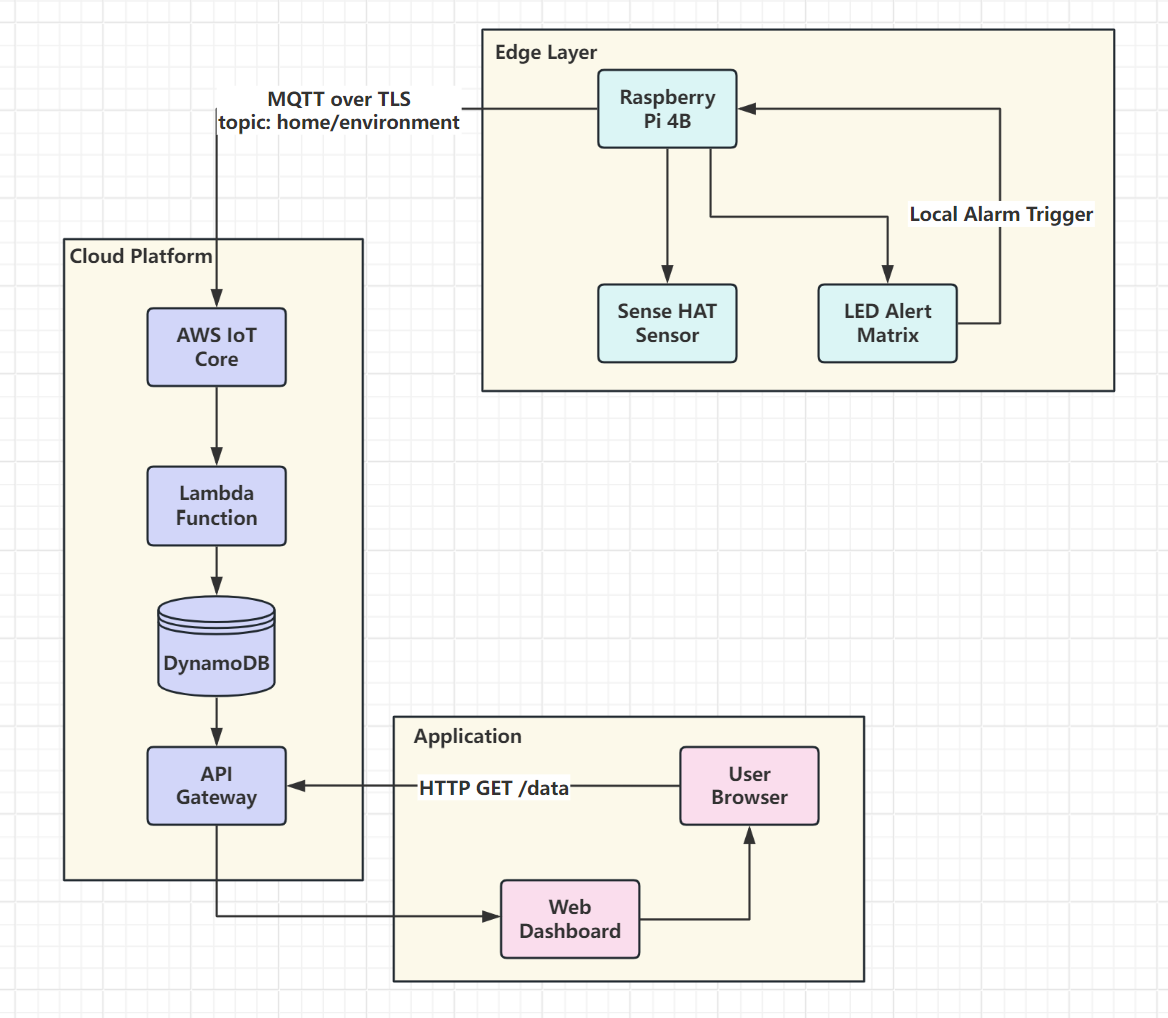
\includegraphics[width=0.75\linewidth]{figures/systemStructure.png}
    \caption{System  Architecture}
\end{figure}


\subsection{Component Selection}
\textbf{Components:}

1. Raspberry Pi 4B

2. Sense HAT Simulator 

\vspace{\baselineskip}
\noindent
\textbf{Cloud Service Configuration:}
The cloud infrastructure is built using the AWS IoT technology stack, with each component working together to enable end-to-end data processing:

\begin{itemize}
    \item \textbf{Device Connectivity Layer:} AWS IoT Core serves as the MQTT message broker, receiving data from edge devices. A minimum-privilege policy named EnvironmentMonitorPolicy is configured to restrict devices to publishing messages only to the $home/environment$ MQTT topic.
    \item \textbf{Data Storage Layer:} A DynamoDB database is deployed, using timestamp (in UNIX format) as the partition key and $device\_id$ as the sort key. Five read/write capacity units are provisioned to support basic throughput performance.
    \item \textbf{Data Processing Layer:} A Lambda function named SaveEnvironmentData handles real-time data processing and persistence. It runs in a Python 3.9 environment and is granted permissions via an execution role named labRole.
    \item \textbf{API Service Layer:} AWS API Gateway is used to expose a RESTful endpoint for cross-origin data access. A GET method is configured to retrieve the latest 20 environmental records.
\end{itemize}


\section{Prototype Implementation}

\subsection{Cloud Backend Architecture}
The edge device publishes sensor data every 5 seconds to the $home/environment$ topic via the MQTT protocol. The AWS IoT Rules Engine listens to this topic in real time and triggers a Lambda function. After data cleansing, the Lambda function stores the processed data into a DynamoDB table. An API Gateway endpoint provides a GET /data interface to retrieve the latest 20 records. The frontend polls this API using AJAX to support real-time visualization.

\begin{figure}[h!]
    \centering
    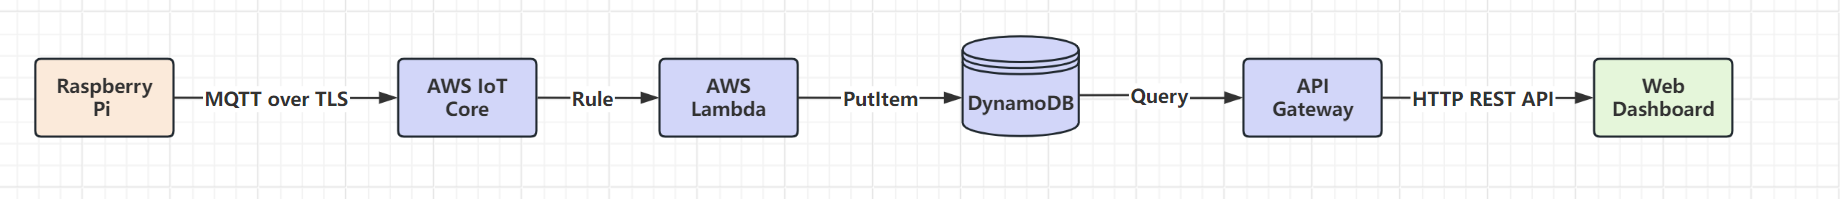
\includegraphics[width=0.95\linewidth]{figures/cloudBackendStructure.png}
    \caption{Cloud Backend  Architecture}
\end{figure}


\subsection{Data Ingestion}

\subsubsection{MQTT Protocol}
Device policy strictly allows publishing to the specified topic only.

\begin{lstlisting}[style=classicpython,caption={mqttToAWS.py snippet},captionpos=b]
    # mqttToAWS.py core code snippet
    def collect_and_publish():
        while True:
            # Sensor data collection
            raw_temp = sense.get_temperature()  
            raw_humi = sense.get_humidity()
            
            # Data cleaning and formatting
            payload = {
                "device_id": "rasip",              
                "temperature": round(raw_temp, 2), 
                "humidity": min(max(raw_humi, 0), 100)  
            }
            
            # MQTT message publishing
            mqtt_connection.publish(
                topic="home/environment",
                payload=json.dumps(payload),
                qos=mqtt.QoS.AT_LEAST_ONCE
            )
            time.sleep(5)  # 5-second data collection cycle
   
        \end{lstlisting}
    

\subsubsection{IoT Rule Configuration}
Rule Name: EnvironmentDataRule

\noindent
SQL Statement: SELECT * FROM 'home/environment'

\noindent
Purpose: Forwards environmental sensor data to a Lambda function for processing.

\begin{figure}[h!]
    \centering
    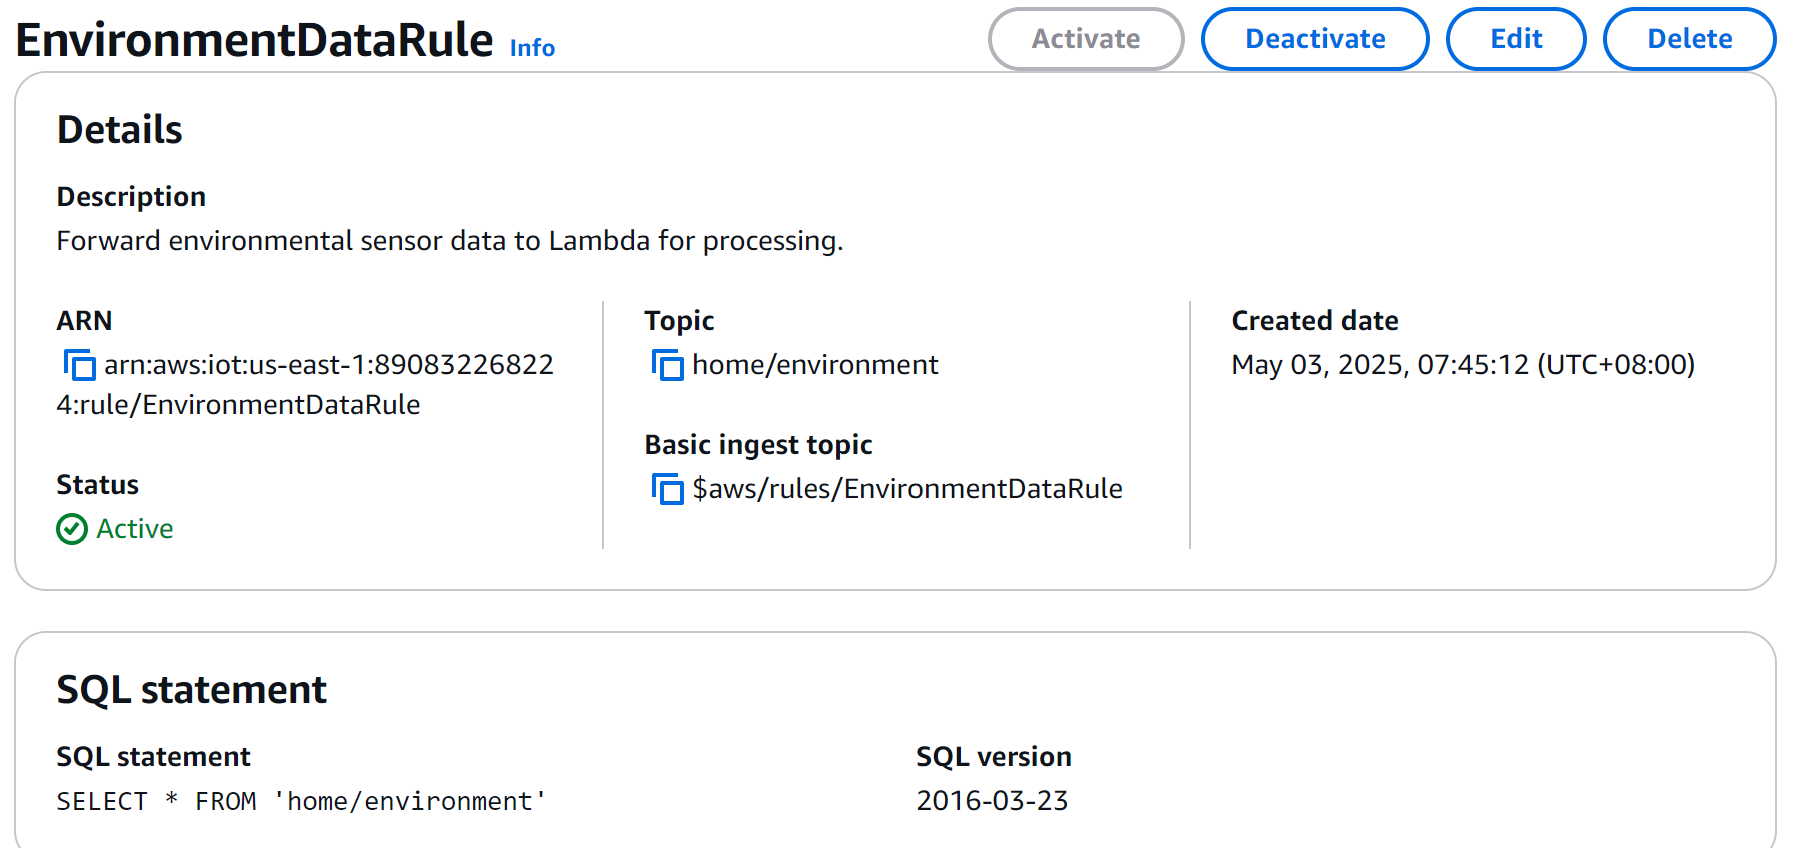
\includegraphics[width=0.95\linewidth]{figures/rule.png}
    \caption{IoT Rule}
\end{figure}



\subsection{Data Processing}
The core logic of the Lambda function SaveEnvironmentData is as follows:

\vspace{\baselineskip}
\noindent
\textbf{1. Receive Raw Data:} Receives MQTT message payload (event) from AWS IoT Core in JSON format, containing temperature, humidity, and $device\_id$.

\vspace{\baselineskip}
\noindent
\textbf{2. Type Conversion and Cleaning:} Converts temperature and humidity to float, ensuring humidity values are within a physically valid range (0\%-100\%) to avoid sensor outliers.

\vspace{\baselineskip}
\noindent
\textbf{3. Precision Handling:} Converts numerical values to the DynamoDB-compatible Decimal type, rounding to two decimal places (e.g., 52.30°C) to prevent precision loss from floating-point values.

\vspace{\baselineskip}
\noindent
\textbf{4. Data Storage:} Stores the processed record, including $device\_id$ and a server-side generated timestamp, into the EnvironmentData\_Maeve DynamoDB table. If any exception occurs (e.g., due to invalid data format), the function returns an HTTP 500 status code and logs the error.

\vspace{\baselineskip}
\begin{lstlisting}[style=classiclambda, caption={Code for Data Processing}]
    import json
    import boto3
    import time
    from decimal import Decimal
    
    
    def lambda_handler(event, context):
        print("Received raw event:", json.dumps(event))
    
        dynamodb = boto3.resource('dynamodb')
        table = dynamodb.Table('EnvironmentData_Maeve')
    
        try:
            payload = event if isinstance(event, dict) else json.loads(event)
    
            temperature = float(payload.get('temperature', 0.0))
            humidity = float(payload.get('humidity', 0.0))
            device_id = payload.get('device_id', 'rasip')
    
            humidity = min(max(humidity, 0.0), 100.0)  
    
            item = {
                'timestamp': int(time.time()),
                'device_id': device_id,
                'temperature': Decimal(str(round(temperature, 2))),
                'humidity': Decimal(str(round(humidity, 2)))
            }
    
            table.put_item(Item=item)
            print("Successfully saved:", item)
            return {'statusCode': 200}
    
        except Exception as e:
            print("Fatal error:", str(e))
            return {'statusCode': 500}
    \end{lstlisting}

    \begin{figure}[h!]
      \centering
      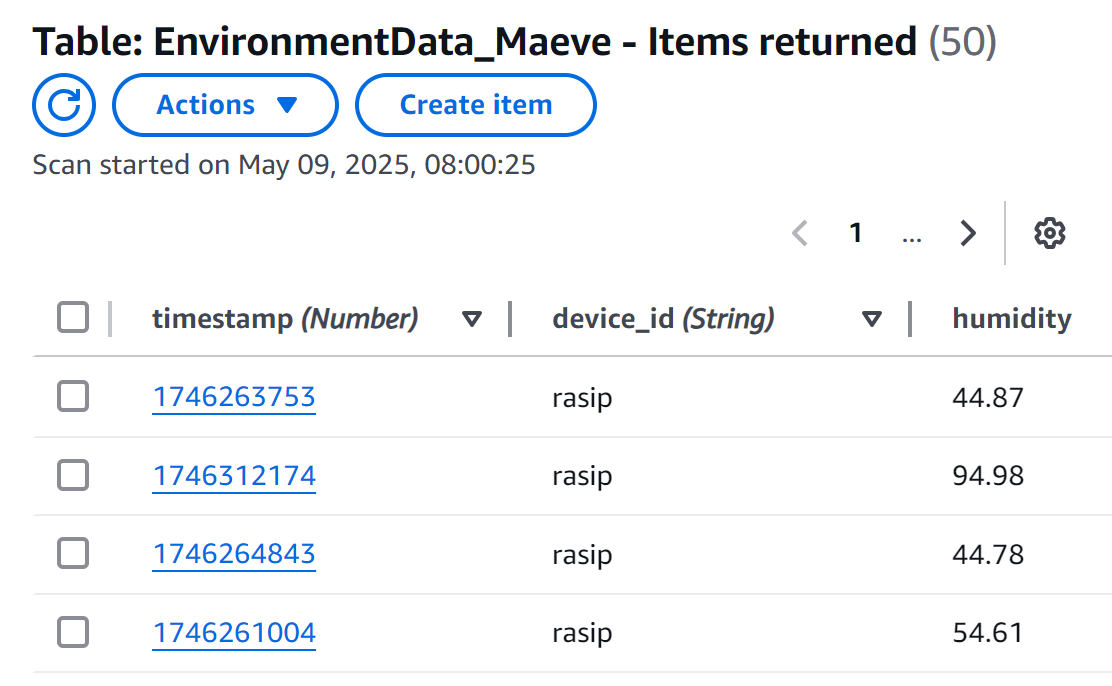
\includegraphics[width=0.58\linewidth]{figures/db.png}
      \caption{EnvironmentData Table Items}
  \end{figure}
  
    
\subsection{Security Implementation}
\subsubsection{ Device Authentication and Communication Security}
\textbf{Implementation Details:}

\noindent
The Raspberry Pi establishes a secure connection with AWS IoT Core using a pre-configured X.509 certificate (located in the $certificates/$ directory). Each certificate contains a unique device identifier and is associated with the AWS IoT policy EnvironmentMonitorPolicy.

\noindent
MQTT communication enforces TLS 1.2 encryption over port 8883. Secure communication is achieved using mqtt\_connection\_builder.mtls\_from\_path in the code.

\vspace{\baselineskip}
\noindent
\textbf{Certificate Rotation:}

\noindent
New certificates can be generated via the AWS IoT Console and used to replace the old ones on the device. The outdated certificate is deactivated to prevent any risk of data leakage.

\subsubsection{ Cloud-Side Access Control}

\textbf{Principle of Least Privilege:}

\vspace{\baselineskip}
\noindent
\textbf{1. Lambda Execution Role:}

\noindent
The Lambda function uses the labRole execution role, which is granted only the dynamodb:PutItem permission (via the managed policy AmazonDynamoDBFullAccess). This ensures that the function can only write to the designated table EnvironmentData\_Maeve.

\vspace{\baselineskip}
\noindent
\textbf{2. IoT Policy Restrictions:}

\noindent
The EnvironmentMonitorPolicy explicitly allows the device to only publish MQTT messages to the topic $home/environment$. All other actions (e.g., subscribe or delete) are denied.

\begin{lstlisting}[language=jsonstyled,caption={Policy in Json},captionpos=b]
    {
        "Version": "2012-10-17",
        "Statement": [
          {
            "Effect": "Allow",
            "Action": "iot:Connect",
            "Resource": "arn:aws:iot:us-east-1:890832268224:client/rasip"
          },
          {
            "Effect": "Allow",
            "Action": "iot:Publish",
            "Resource": "arn:aws:iot:us-east-1:890832268224:topic/home/environment"
          }
        ]
      }
    \end{lstlisting}

\subsection{UI Features}

\subsubsection{Real-Time Data Visualization}
The frontend uses the ApexCharts library to dynamically render temperature and humidity line charts, implementing the following features:

\vspace{\baselineskip}
\noindent
\textbf{Data Fetching:} JavaScript calls the $fetchData()$ function to retrieve the latest 20 records from the API Gateway endpoint (https://toxyu2j8cc.../dev/data), displaying them in reverse chronological order.

\vspace{\baselineskip}
\noindent
\textbf{Chart Updating:} The $chart.updateSeries()$ method is invoked to refresh the chart in real-time. If the temperature exceeds 50°C, the temperature line switches to red; if the humidity exceeds 80\%, the humidity line switches to blue (as defined in the updateChartData function in $script.js$).

\vspace{\baselineskip}
\noindent
\textbf{Timestamp Handling:} The X-axis converts UNIX timestamps (in milliseconds) into local time format to prevent timezone-related confusion.

\subsubsection{Alert Status Indication}
\textbf{Status Banner:} The top banner dynamically changes style based on alert conditions:


\begin{figure}[h!]
  \centering
  \begin{subfigure}[b]{0.46\textwidth}
      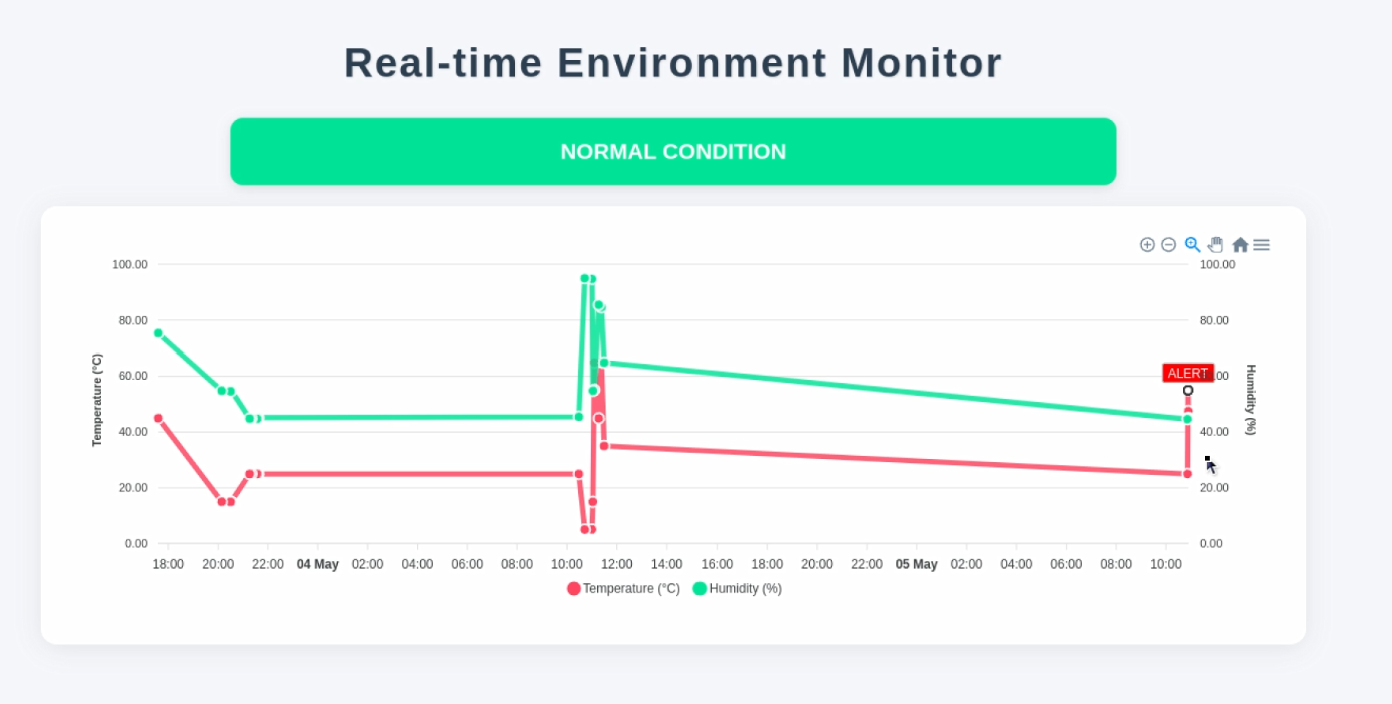
\includegraphics[width=\textwidth]{figures/1.png}
      \caption{Normal Condition}
      \label{fig:sub1}
  \end{subfigure}
  \hfill
  \begin{subfigure}[b]{0.46\textwidth}
      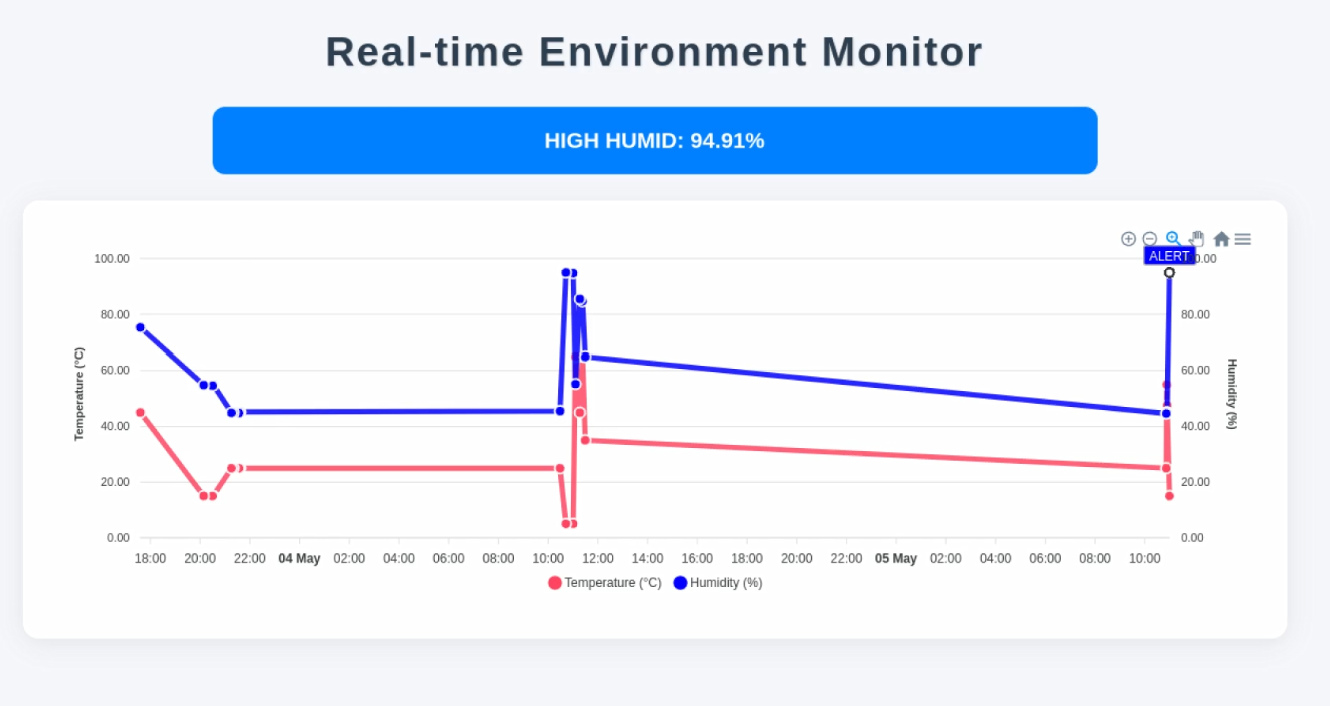
\includegraphics[width=\textwidth]{figures/2.png}
      \caption{High Humidity}
      \label{fig:sub2}
  \end{subfigure}
  
  \vspace{0.5cm} % 图行间距
  
  \begin{subfigure}[b]{0.46\textwidth}
      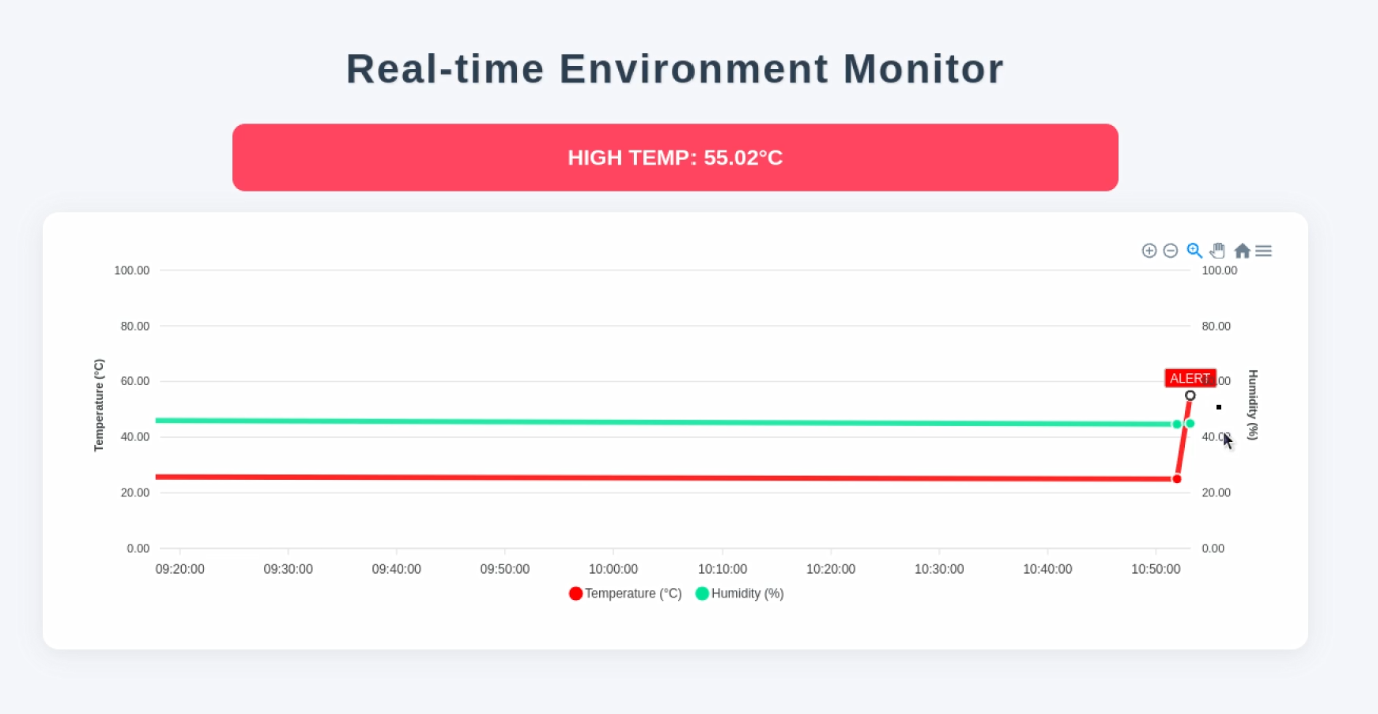
\includegraphics[width=\textwidth]{figures/3.png}
      \caption{High Temperature}
      \label{fig:sub3}
  \end{subfigure}
  \hfill
  \begin{subfigure}[b]{0.46\textwidth}
      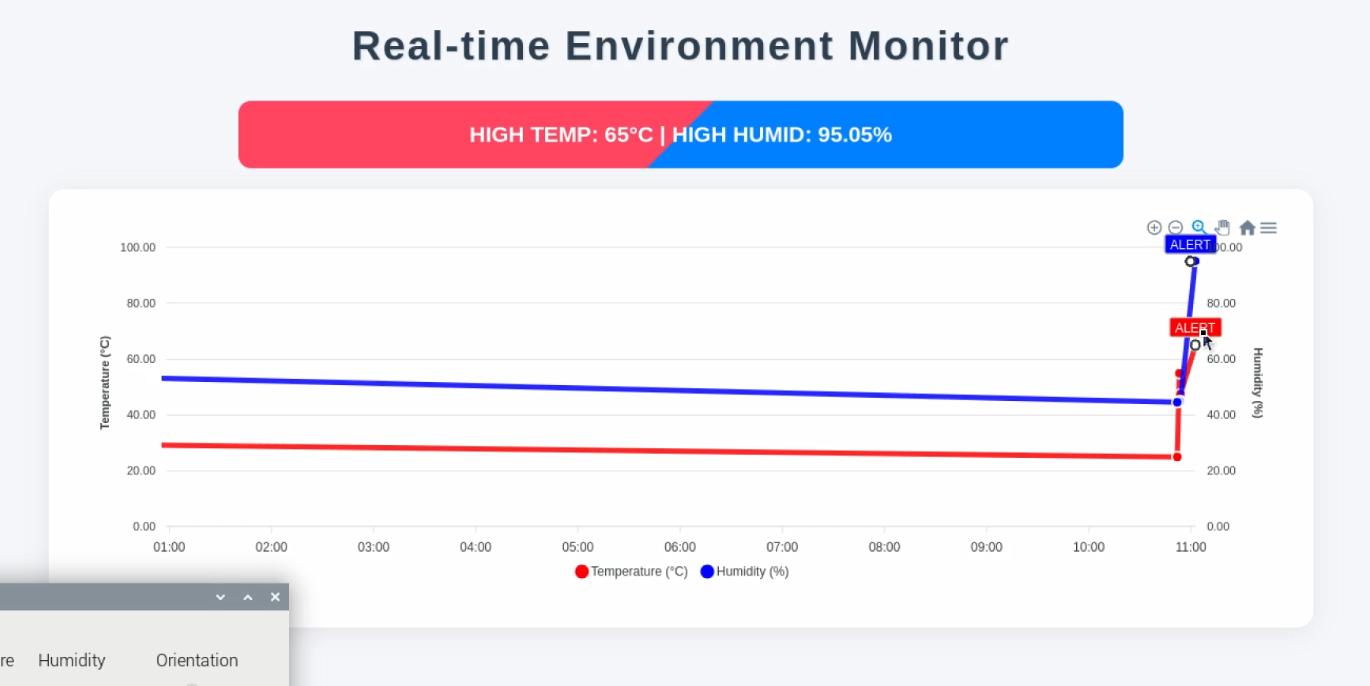
\includegraphics[width=\textwidth]{figures/4.png}
      \caption{Dual Alert}
      \label{fig:sub4}
  \end{subfigure}
  
  \caption{Frontend Alert}
  \label{fig:allplots}
\end{figure}


\vspace{\baselineskip}
\noindent
\textbf{Chart Annotation:} When the latest data point exceeds the defined threshold, the chart dynamically adds an "ALERT" label using $chart.addPointAnnotation()$ (red or blue).

\vspace{\baselineskip}
\noindent
\textbf{Device-Level Detection:} On the device side, $mqttToAWS.py$ directly controls the LED alert system via the $set\_alarm\_led()$ function. It activates red or blue LED text alerts when temperature exceeds 50°C or humidity exceeds 80\%, respectively.


\begin{figure}[h!]
  \centering
  \begin{subfigure}[b]{0.31\textwidth}
      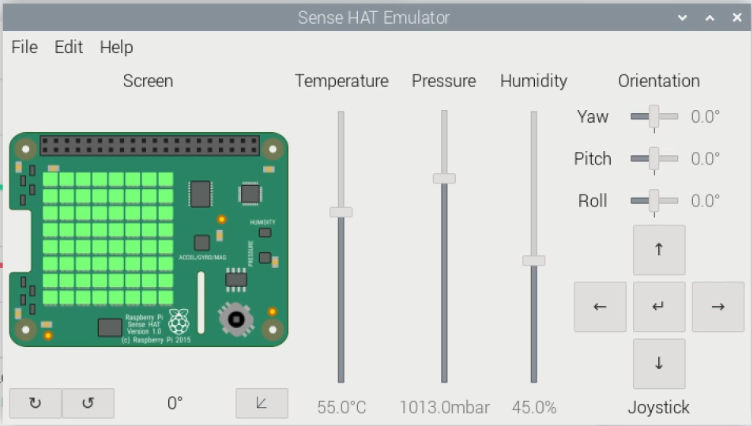
\includegraphics[width=\textwidth]{figures/11.png}
      \caption{Normal Condition}
      \label{fig:sub1}
  \end{subfigure}
  \hfill
  \begin{subfigure}[b]{0.31\textwidth}
      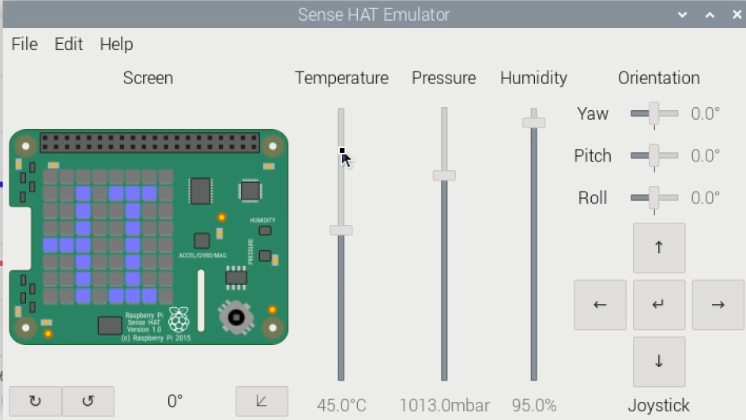
\includegraphics[width=\textwidth]{figures/22.png}
      \caption{High Humidity}
      \label{fig:sub2}
  \end{subfigure}
  \hfill
  \begin{subfigure}[b]{0.31\textwidth}
      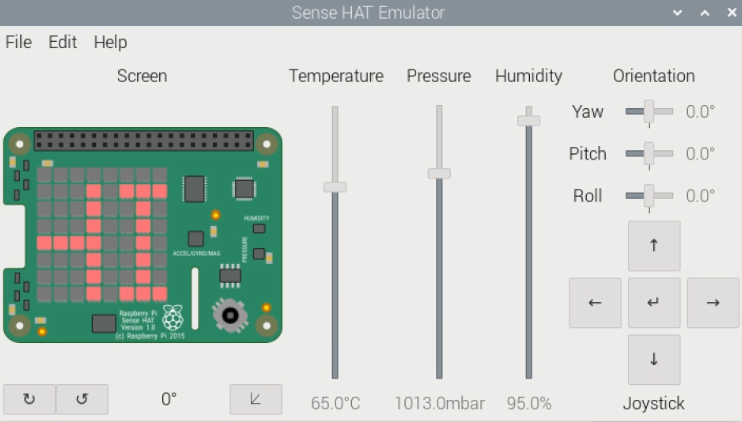
\includegraphics[width=\textwidth]{figures/33.png}
      \caption{High Temperature}
      \label{fig:sub3}
  \end{subfigure}
  \caption{Device Alert}
  \label{fig:upload-stages}
\end{figure}

\subsubsection{User Authentication System}

On first access, a dialog prompts the user to enter a username and password. Upon successful verification, the authentication state is stored via $localStorage.setItem()$.

\begin{figure}[h!]
  \centering
  \begin{subfigure}[b]{0.45\textwidth}
      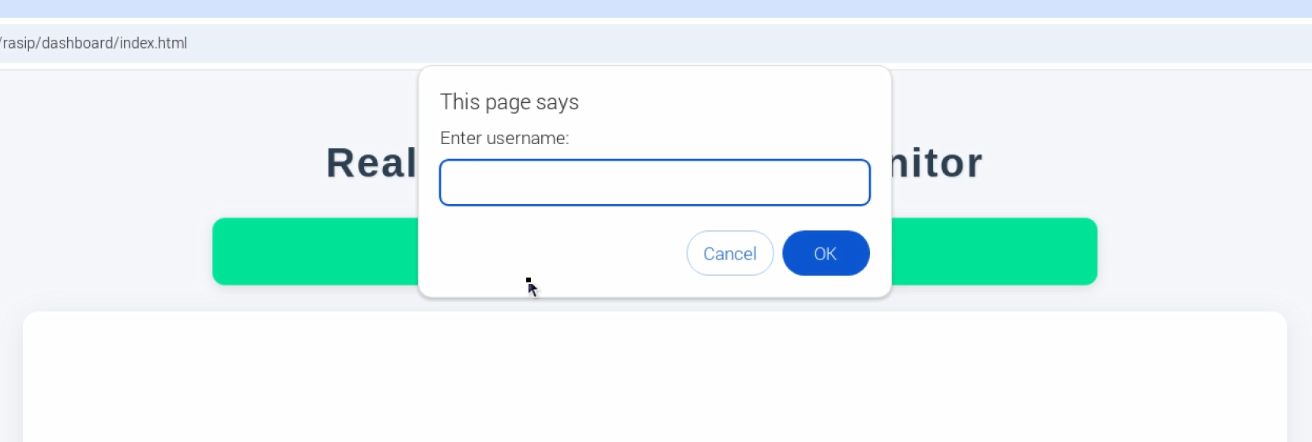
\includegraphics[width=\textwidth]{figures/userName.png}
      \caption{Enter UserName}
      \label{fig:twoimg1}
  \end{subfigure}
  \hfill
  \begin{subfigure}[b]{0.45\textwidth}
      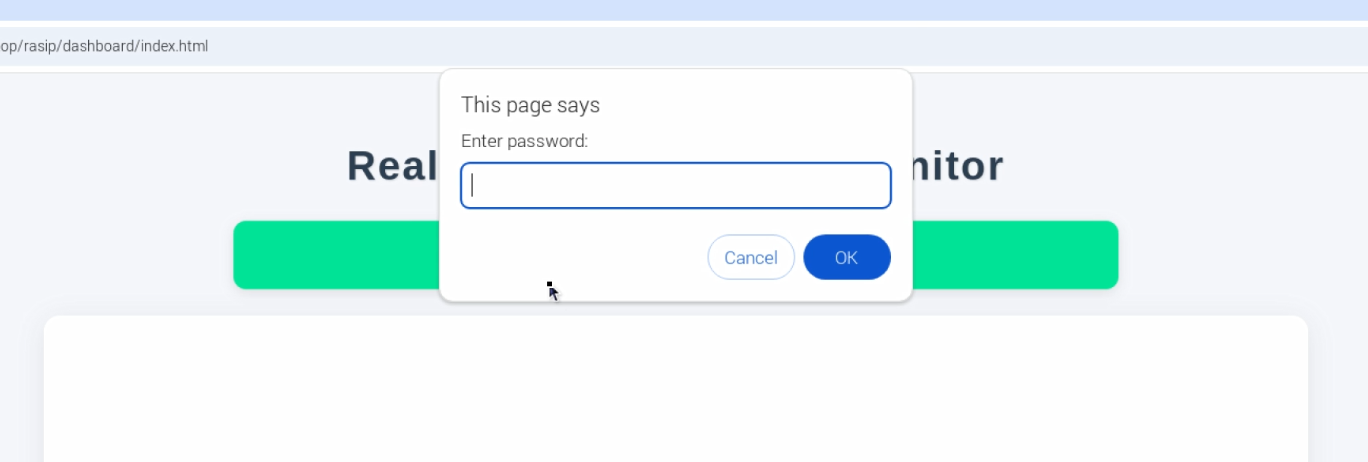
\includegraphics[width=\textwidth]{figures/pw.png}
      \caption{Enter Password}
      \label{fig:twoimg2}
  \end{subfigure}
  \caption{Authentication Check}
  \label{fig:twoimageset}
\end{figure}

\vspace{\baselineskip}
\noindent
The login status is checked using $localStorage.getItem('env\_monitor\_auth')$. Unauthenticated users are blocked from viewing data and are forced to refresh the page.

\vspace{\baselineskip}
\noindent
This authentication method is intended for development and testing purposes only. Credentials are transmitted and stored in plain text, with no HTTPS encryption or server-side validation implemented.




\begin{lstlisting}[style=classicpython,caption={checkAuth Code Snippet},captionpos=b]
  function checkAuth() {
      if (!localStorage.getItem('env_monitor_auth')) {
        const username = prompt('Enter username:'); 
        const password = prompt('Enter password:'); 
        if (username === 'admin' && password === 'admin123') {
          localStorage.setItem('env_monitor_auth', 'authenticated');
        }
      }
    }
    
  \end{lstlisting}



\subsection{Data Analytics}
To verify the integrity of system-collected data and analyze temperature and humidity trends, this project utilizes the AWS DynamoDB console and CloudWatch Logs Insights for basic querying and visualization.

\vspace{\baselineskip}
\noindent
First go to DynamoDB and run the following query to retrieve the 20 most recent records, ensuring the device is uploading data correctly:
\begin{lstlisting}[style=maevesql, caption={query the data}]
  SELECT * FROM "EnvironmentData_Maeve"
  WHERE device_id = 'rasip'
  ORDER BY timestamp DESC 
  LIMIT 20;  
\end{lstlisting}


\noindent
Then go the CloudWatch console and navigate to Logs Insights. Use the query to calculate average temperature and humidity, grouped by 5-minute intervals across the most recent 100 logs.
\begin{lstlisting}[style=maevesql, caption={query the data}]
  fields @timestamp, temperature, humidity
  | sort @timestamp desc
  | limit 100
  | stats avg(temperature) as avg_temp, avg(humidity) as avg_humi by bin(5m)
\end{lstlisting}

Below is the chart generated by CloudWatch Visualize function.

\begin{figure}[h!]
  \centering
  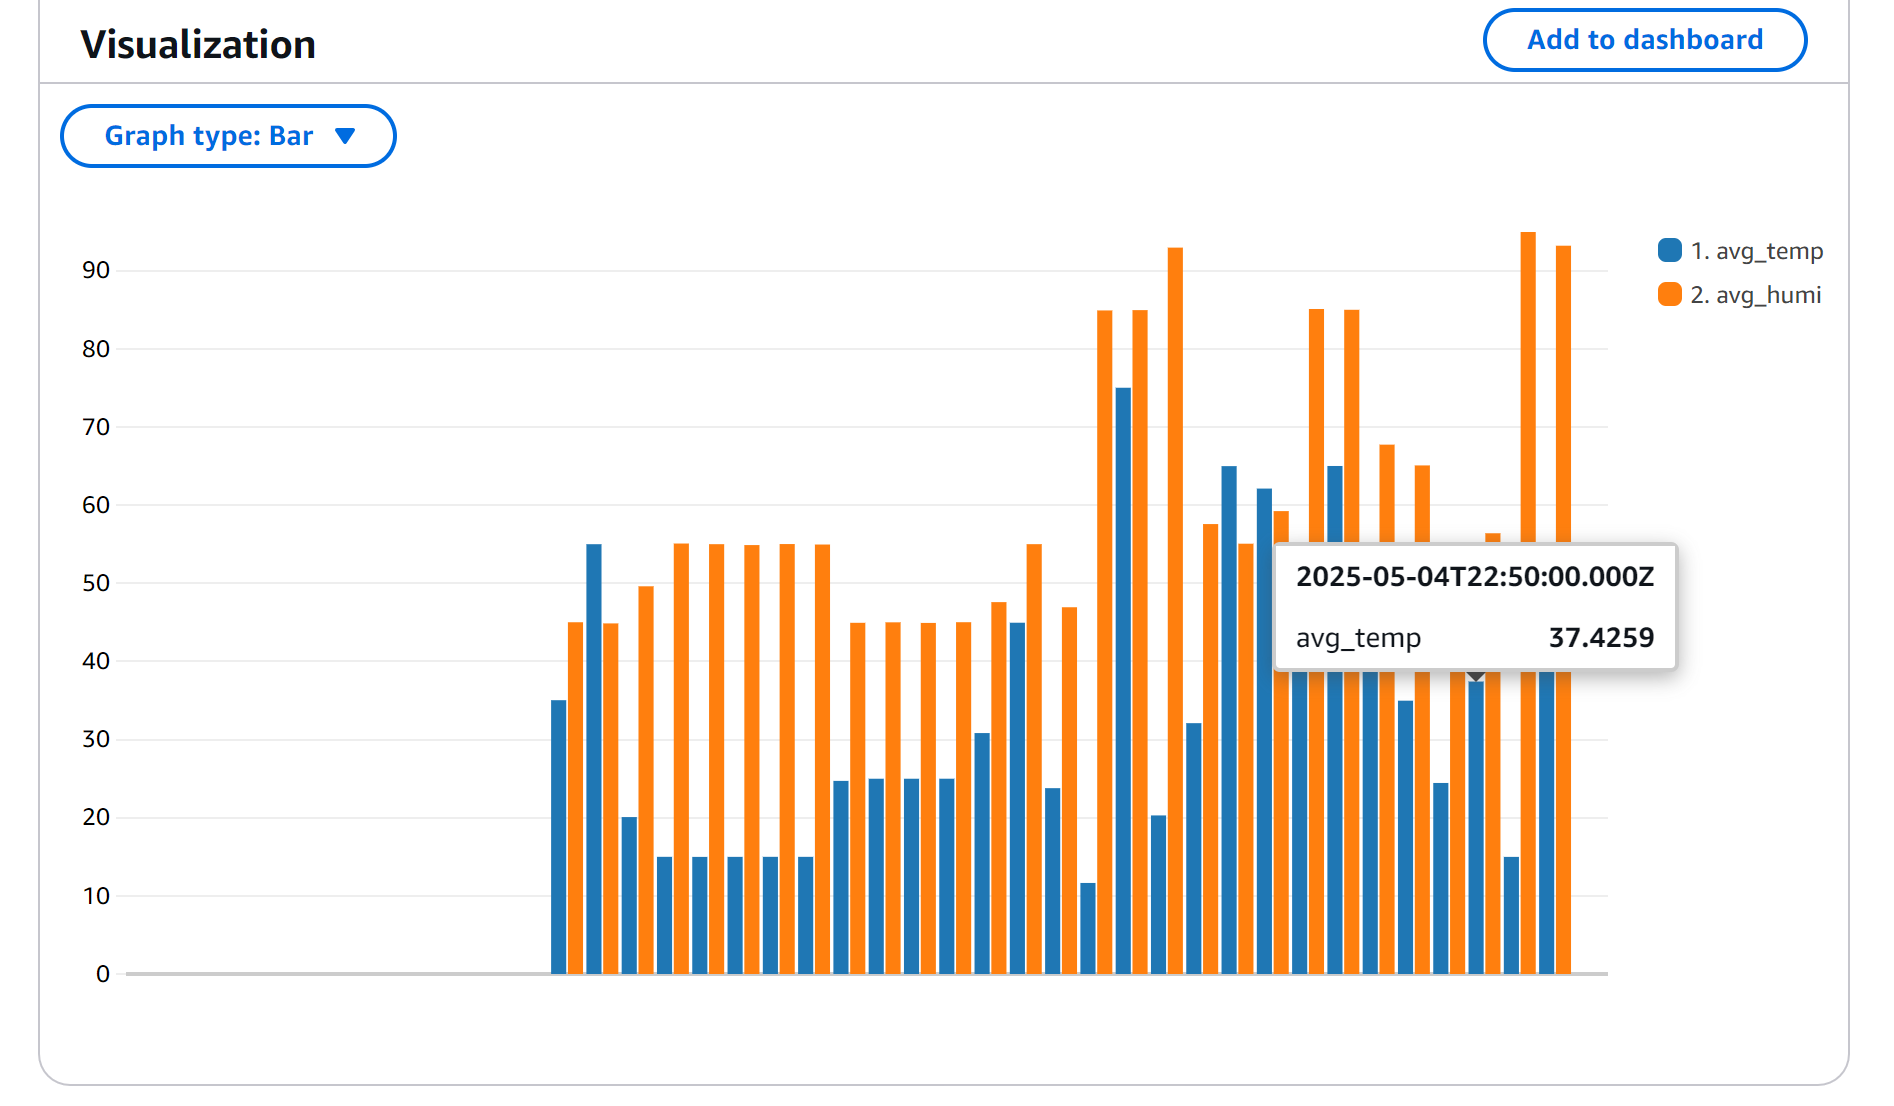
\includegraphics[width=0.75\linewidth]{figures/analysis.png}
  \caption{CloudWatch Logs Insight}
\end{figure}

\subsection{Real-Time Trend Visualization}
The frontend dynamically displays temperature and humidity trends using ApexCharts line charts. Users can zoom in on specific time ranges (e.g., past 1 hour or 24 hours) to explore data.

\vspace{\baselineskip}
\noindent
Interactive tooltips show precise values and timestamps on hover, aiding manual analysis of abnormal periods.


\section{Deployment Guide}

\subsection{Hardware Configuration}
The Raspberry Pi runs a pre-installed Raspberry Pi OS on a microSD card. It executes the $mqttToAWS.py$ Python script for data collection and transmission.

\vspace{\baselineskip}
\noindent
Dependencies: awsiotsdk (install via pip3 install)

\vspace{\baselineskip}
\noindent
Sense HAT simulator (install via sudo apt-get install sense-hat)

\vspace{\baselineskip}
\noindent
The device certificate files (.pem format) are stored in the $certificates/$ directory. The script must explicitly specify the paths to the device certificate, private key, and root CA to ensure a secure MQTT connection over TLS 1.2 to the AWS IoT Core endpoint: a18s752r9nbkhs-ats.iot.us-east-1.amazonaws.com.

\vspace{\baselineskip}
\noindent
Below is my project structure:

\begin{lstlisting}[language=,basicstyle=\ttfamily]
  project_root/
  |-- mqttToAWS.py        # Data transmission script
  |-- certificates/       # Certificate files
  |   |-- AmazonRootCA1.pem
  |   |-- AmazonRootCA3.pem
  |   |-- certificate.pem.crt
  |   |-- public.pem.key
  |   |-- private.pem.key
  |-- dashboard/          # Web dashboard files
  |   |-- index.html      # Main interface
  |   |-- script.js       # Data fetching logic
  \end{lstlisting}

  
\subsection{Cloud Deployment}
Register the device in AWS IoT Core and attach the EnvironmentMonitorPolicy, allowing the device to publish only to the $home/environment$ topic.

\vspace{\baselineskip}
\noindent
Create a DynamoDB table named $EnvironmentData_Maeve$ with $timestamp$ (Number) and $device\_id$ (String) as the primary key.

\vspace{\baselineskip}
\noindent
Set up a Lambda function SaveEnvironmentData (runtime: Python 3.9), triggered by an IoT Rule, with execution role labRole to enable data insertion.

\vspace{\baselineskip}
\noindent
Use API Gateway to create a REST endpoint: https://toxyu2j8cc.execute-api.us-east-1.amazonaws.com/dev/data, integrated with the SimpleDataQuery Lambda function to provide data query functionality.


\subsection{Frontend Deployment}
The static frontend files ($index.html$ and $script.js$) can be run locally using Python's built-in HTTP server: python3 -m http.server 8000

\vspace{\baselineskip}
\noindent
Alternatively, they can be hosted on any HTTPS-enabled web server.

\vspace{\baselineskip}
\noindent
The frontend fetches data from the hardcoded API Gateway URL and manages authentication status using localStorage. The login credentials are fixed as admin/admin123.

\subsection{Verification Process}
After launching $mqttToAWS.py$, verify terminal output for "Connected!" and log entries for data publication on the Raspberry Pi.

\vspace{\baselineskip}
\noindent
In the AWS DynamoDB console, check for new entries.

\vspace{\baselineskip}
\noindent
Open the frontend page to confirm that the charts are updating in real-time and that alert statuses are displayed.

\vspace{\baselineskip}
\noindent
If anomalies are detected, inspect the Lambda logs in CloudWatch and verify the certificate permissions on the device side.

\section{User Manual}

\subsection{System Startup}
Power On the Device: Connect the Raspberry Pi to a power source. The system will automatically boot, then run the $mqttToAWS.py$ script.

\noindent
Status Confirmation: Check the Raspberry Pi’s LED matrix display:

\begin{itemize}
  \item Solid Green: System is running normally and data is being uploaded.
  \item Scrolling Red Text: Temperature exceeds 50°C.
  \item Scrolling Blue Text: Humidity exceeds 80\%
\end{itemize}

\subsection{Accessing the Dashboard}
Open $index.html$ directly in a browser.

\noindent
Login Authentication: On first access, enter the username admin and password admin123.

\subsection{Interface Features}
Real-Time Chart:
\begin{itemize}
  \item Red Line: Temperature (°C). Turns red and displays an "ALERT" tag if it exceeds 50°C.
  \item Blue Line: Humidity (\%). Turns blue and displays an "ALERT" tag if it exceeds 80\%.
  \item Zooming: Click and drag the chart area to explore historical data in detail.
\end{itemize}

\noindent
Status Panel:

\begin{itemize}
  \item Green: Environment is normal.
  \item Red: Temperature alert (shows current value).
  \item Blue: Humidity alert (shows current value).
  \item Red-Blue Gradient: Both temperature and humidity exceed thresholds.
\end{itemize}

\subsection{Alert Handling}
Local Alert:

\noindent
1. If the LED matrix displays scrolling text, check for ventilation or dehumidification needs.

\noindent
2. Once the alert condition is resolved, the LED will automatically return to solid green.

\noindent
Remote Notification:

\noindent
1. The top status bar of the dashboard continuously shows active alerts.

\noindent
2. Press F5 to manually refresh and retrieve the latest status.

\subsection{Troubleshooting}

\begin{table}[h!]
\centering
\renewcommand{\arraystretch}{1.3}  
\setlength{\tabcolsep}{10pt}      
\begin{tabular}{|p{5cm}|p{9cm}|}
\hline
\textbf{Issue} & \textbf{Solution} \\
\hline
Cannot log in & Confirm correct credentials (\texttt{admin/admin123}), clear browser cache. \\
\hline
No data in chart & Check device power and internet connection, wait 1–2 minutes. \\
\hline
Status bar shows ``Connection Failed'' & Verify the configured API Gateway URL is correct. \\
\hline
LED matrix not lit & Restart the Raspberry Pi and ensure \texttt{mqttToAWS.py} is running. \\
\hline
\end{tabular}
\caption{Troubleshooting Common Issues}
\label{tab:troubleshooting}
\end{table}



% \newpage
% \begin{thebibliography}{99}

%     \bibitem{1}
%     Alliance, A. (2017). Agile Practice Guide, Project Management Institute, 2017: Agile Practice Guide (Vol. 1). Bukupedia.

%     \bibitem{2}
%     Highsmith, J. A. (2010). Agile project management : creating innovative products (2nd ed ed.). Addison-Wesley.
%     \end{thebibliography}





\end{document}
